\let\negmedspace\undefined
\let\negthickspace\undefined
\documentclass[journal]{IEEEtran}
\usepackage[a5paper, margin=10mm, onecolumn]{geometry}
%\usepackage{lmodern} % Ensure lmodern is loaded for pdflatex
\usepackage{tfrupee} % Include tfrupee package

\setlength{\headheight}{1cm} % Set the height of the header box
\setlength{\headsep}{0mm}     % Set the distance between the header box and the top of the text

\usepackage{gvv-book}
\usepackage{gvv}
\usepackage{cite}
\usepackage{amsmath,amssymb,amsfonts,amsthm}
\usepackage{algorithmic}
\usepackage{graphicx}
\usepackage{textcomp}
\usepackage{xcolor}
%\usepackage{txfonts}
\usepackage{listings}
\usepackage{enumitem}
\usepackage{mathtools}
\usepackage{gensymb}
\usepackage{comment}
\usepackage[breaklinks=true]{hyperref}
\usepackage{tkz-euclide} 
\usepackage{listings}
% \usepackage{gvv}                                        
\def\inputGnumericTable{}                                 
\usepackage[latin1]{inputenc}                                
\usepackage{color}                                            
\usepackage{array}                                            
\usepackage{longtable}                                       
\usepackage{calc}                                             
\usepackage{multirow}                                         
\usepackage{hhline}                                           
\usepackage{ifthen}                                           
\usepackage{lscape}
\usepackage{circuitikz}
\tikzstyle{block} = [rectangle, draw, fill=blue!20, 
    text width=4em, text centered, rounded corners, minimum height=3em]
\tikzstyle{sum} = [draw, fill=blue!10, circle, minimum size=1cm, node distance=1.5cm]
\tikzstyle{input} = [coordinate]
\tikzstyle{output} = [coordinate]


\begin{document}

\bibliographystyle{IEEEtran}
\vspace{3cm}

\title{5.8.11}
\author{EE25BTECH11013 - Bhargav}
\maketitle
{\let\newpage\relax\maketitle}

\renewcommand{\thefigure}{\theenumi}
\renewcommand{\thetable}{\theenumi}
\setlength{\intextsep}{10pt} % Space between text and floats

\numberwithin{equation}{enumi}
\numberwithin{figure}{enumi}
\renewcommand{\thetable}{\theenumi}

\textbf{Question}:\\
The coach of a cricket team buys $3$ bats and $6$ balls for \rupee 3900. Later, she buys
another bat and $3$ more balls of the same kind for \rupee 3300. Find the cost of a bat and
ball.

\solution \\

Let the cost of the bat, ball be \rupee x and \rupee y respectively.
\begin{align}
\myvec{3 & 6}\myvec{x \\ y} = 3900
\end{align}
\begin{align}
\myvec{1 & 3}\myvec{x \\ y} = 3300
\end{align}

These can be combined to give the matrix equation
\begin{align}
\myvec{3 & 6 \\ 1 & 3}\myvec{x \\ y} = \myvec{3900 \\ 3300}
\end{align}

This gives the augmented matrix
\begin{align}
\augvec{2}{1}{3 & 6 & 3900 \\ 1 & 3 & 3300} \xleftrightarrow{R_2 \leftarrow R_2 - \frac{1}{3}R_1} \augvec{2}{1}{3 & 6 & 3900 \\ 0 & 1 & 2000}
\end{align}

This gives the following values of x and y:
\begin{align}
\myvec{x \\ y} = \myvec{-2700 \\ 2000}
\end{align}

Thus, the cost of one ball is \rupee 2000 and the cost of one bat is - \rupee 2700

\begin{figure}[h!]
    \centering
    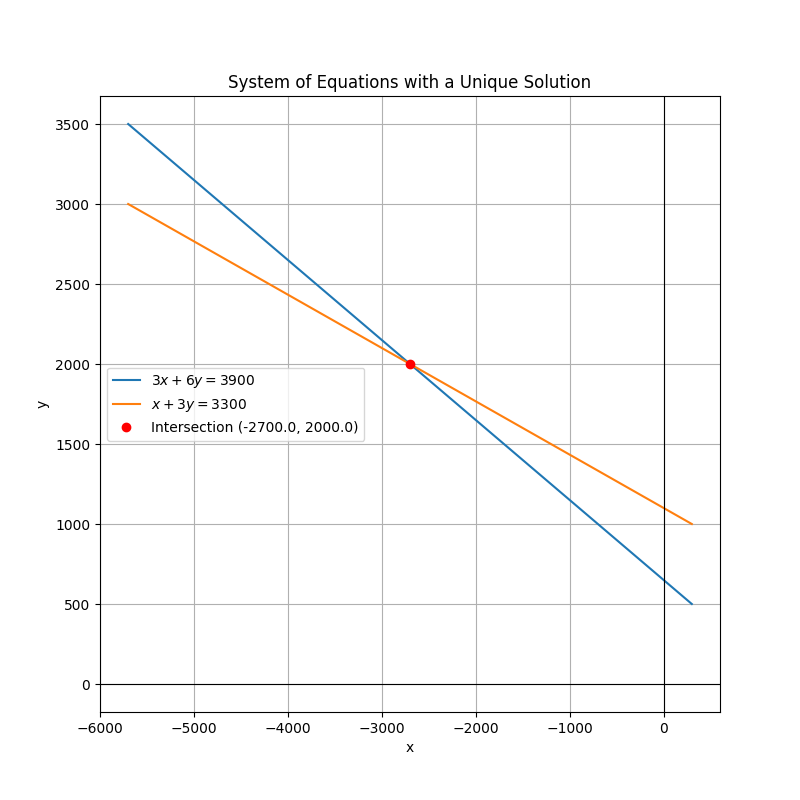
\includegraphics[height=0.5\textheight, keepaspectratio]{figs/Figure_1.png}
    \label{figure_1}
\end{figure}
\end{document}